% ==========================================================
% Póster académico A1 horizontal · 3 columnas (referencias al final de la última)
% Maestría en Inteligencia Artificial Aplicada
%
% Basado en poster_plantilla: se conservan encabezado, paleta, barras de
% sección, tipografías y tamaños de la plantilla. Solo se reemplaza el
% contenido de ejemplo (lipsum / imágenes de ejemplo).
%
% Compilación:
%   - pdfLaTeX (por defecto): Charter para títulos.
%   - XeLaTeX / LuaLaTeX: "Instrument Serif" para títulos si está
%     instalada (o subida a Overleaf); si no, TeX Gyre Pagella.
% Archivos necesarios: carpeta figs/ y, opcionalmente, logo.jpeg / logo_der.png
% ==========================================================
\documentclass[10pt]{article}
\usepackage{iftex}
\usepackage[a1paper,landscape,margin=1.5cm]{geometry}
\usepackage[spanish,es-noshorthands]{babel}
\usepackage{xcolor}
\usepackage{graphicx}
\usepackage{tikz}
\usetikzlibrary{arrows.meta}
\usepackage[most]{tcolorbox}
\usepackage{enumitem}
\usepackage{booktabs}
\usepackage{colortbl}
\usepackage{microtype}
% ---------------------- TIPOGRAFÍA -------------------------
% Texto: fuente por defecto (Latin Modern). Títulos: \serif.
\ifTUTeX
  \usepackage{fontspec}
  \IfFontExistsTF{Instrument Serif}%
    {\newfontfamily\serif{Instrument Serif}}%
    {\newfontfamily\serif{TeX Gyre Pagella}}
\else
  \usepackage[utf8]{inputenc}
  \usepackage[T1]{fontenc}
  \usepackage{lmodern}      % fuentes escalables (evita avisos de tamaños)
  \usepackage[scaled=0.95]{helvet}
  \newcommand{\serif}{\fontfamily{bch}\selectfont}
\fi
\pagestyle{empty}
\setlength{\parindent}{0pt}
\setlength{\parskip}{0.4em}
% ---------------------- PALETA -----------------------------
\definecolor{olive}{HTML}{9AA542}        % encabezados de sección
\definecolor{olivedark}{HTML}{1B2208}    % títulos / texto de encabezados
\definecolor{olivelink}{HTML}{6B7A1F}    % acentos
\definecolor{olivesoft}{HTML}{E4E8C7}    % círculos / fondos suaves
\definecolor{ink}{HTML}{1A1A10}          % texto
\definecolor{muted}{HTML}{6B6B5E}
\definecolor{pagebg}{HTML}{FFFFFF}       % usa F8F8F3 para fondo crema
\definecolor{alerta}{HTML}{B5462B}       % acento para resultados negativos (gráficas)
\pagecolor{pagebg}
\color{ink}
% ---------------------- DATOS DEL PÓSTER -------------------
\newcommand{\programa}{Maestría en Inteligencia Artificial Aplicada}
\newcommand{\tituloA}{Clasificación morfológica de galaxias mediante fusión multimodal}
\newcommand{\tituloB}{de imágenes, espectroespectros y poblaciones estelares}
\newcommand{\autores}{Alexander Carreño\quad Julio Ricardo Velázquez\quad María Rabelero}
\newcommand{\asesor}{Dr. José Antonio Vázquez Mata y Dr. Héctor Manuel Hernández Toledo}
\newcommand{\fecha}{Noviembre 2026}
% Logos (archivos: logo.jpeg / logo_der.png)
% Si no se permite la incorporación del logo de la empresa, usar el de MNA incluido en la carpeta
\newcommand{\logoizq}{%
  \IfFileExists{figs/logo.jpeg}%
  {
\includegraphics[height=3.5cm]{figs/logo.jpeg}}%
  {\tikz\node[draw=olive,dashed,line width=1.2pt,minimum width=10cm,
    minimum height=6cm,align=center,text=muted]{\Huge LOGO\\IZQUIERDO};}}
\newcommand{\logoder}{%
  \IfFileExists{figs/logo_unam.png}%
  {
\includegraphics[height=5cm]{figs/logo_unam.png}}%
  {\tikz\node[draw=olive,dashed,line width=1.2pt,minimum width=10cm,
    minimum height=6cm,align=center,text=muted]{\Huge LOGO EMPRESA\\DERECHO};}}
% ---------------------- ESTILOS ----------------------------
% Barra de sección (serif, texto oscuro sobre verde)
\newcommand{\seccion}[1]{%
  \begin{tcolorbox}[colback=olive,colframe=olive,arc=0pt,
    boxrule=0pt,left=8pt,top=3pt,bottom=4pt,width=\linewidth]
    {\serif\color{white}\fontsize{30}{36}\selectfont #1}
  \end{tcolorbox}\vspace{-0.3em}}
% Texto base (fuente por defecto de LaTeX)
\newcommand{\cuerpo}{\fontsize{24}{31}\selectfont}
% Pie de figura
\newcommand{\pie}[1]{{\sffamily\fontsize{18}{22}\selectfont\color{muted}#1}}
% Indicador (número grande + etiqueta)
\newcommand{\kpi}[3]{%
  \colorbox{#3}{\parbox[c][4.3cm][c]{\dimexpr0.24\linewidth-2\fboxsep\relax}{\centering
    {\serif\fontsize{58}{62}\selectfont\color{olivedark}#1}\\[0.15em]
    {\sffamily\bfseries\fontsize{19}{23}\selectfont\color{olivedark}#2}}}}
% Indicador: número grande + línea 1 (negrita) + línea 2 (normal) 
% \kpi[color]{número}{línea 1 en negrita}[línea 2 normal] 
%\NewDocumentCommand{\kpi}{O{olivesoft} m m o}{% 
%  \colorbox{#1}{\parbox[c][4.3cm][c]{\dimexpr0.24\linewidth-2\fboxsep\relax}{\centering 
%    {\serif\fontsize{58}{62}\selectfont\color{olivedark}#2}\\[0.15em] 
%    {\sffamily\fontsize{16}{20}\selectfont\color{olivedark}% 
%      {\bfseries #3}\IfValueT{#4}{\\#4}}}}}
% Mensaje destacado
\newcommand{\clave}[1]{%
  \colorbox{olivesoft}{\parbox{\dimexpr\linewidth-2\fboxsep\relax}{\fontsize{22}{28}\selectfont\color{olivedark}#1}}}
% Alturas del diseño (ajusta si cambias el tamaño del encabezado)
\newlength{\hdrh}\setlength{\hdrh}{9cm}      % encabezado
\newlength{\colh}
\setlength{\colh}{\dimexpr\textheight-\hdrh-3.5cm\relax}
\setlist[itemize]{leftmargin=1.2em,itemsep=0.25em,topsep=0.2em,parsep=0pt}
% ======================================================
\begin{document}
% ---------------------- ENCABEZADO ------------------------
\noindent\parbox[t][\hdrh][c]{\linewidth}{%
\begin{minipage}[c]{0.10\linewidth}
  \raggedright\logoizq
\end{minipage}%
\begin{minipage}[c]{0.80\linewidth}
  \centering
  {\serif\fontsize{58}{65}\selectfont\color{olivedark}%
   \tituloA\\\tituloB\par}
  \vspace{0.5em}
  {\sffamily\bfseries\fontsize{30}{36}\selectfont\color{olivelink}\programa\par}
  \vspace{0.3em}
  {\fontsize{26}{32}\selectfont\color{ink}\autores\par}
  {\fontsize{22}{28}\selectfont\color{muted}Asesores: \asesor\ \textperiodcentered\ \fecha\par}
\end{minipage}%
\begin{minipage}[c]{0.10\linewidth}
  \raggedleft\logoder
\end{minipage}}
\vspace{0.4cm}
{\color{olive}\rule{\linewidth}{2.5pt}}
\vspace{0.6cm}
% ---------------------- COLUMNAS --------------------------
\noindent
\begin{minipage}[t][\colh][s]{0.30\linewidth}\cuerpo\vspace{0pt}
% ===== COLUMNA IZQUIERDA =====
\seccion{Problema: Clasificar morfologías a gran escala}
Se clasifican manualmente 10,059 galaxias MaNGA. ¿Pueden imagen, espectro y poblaciones \textbf{imitar a un experto} en clasificación?
\begin{center}
  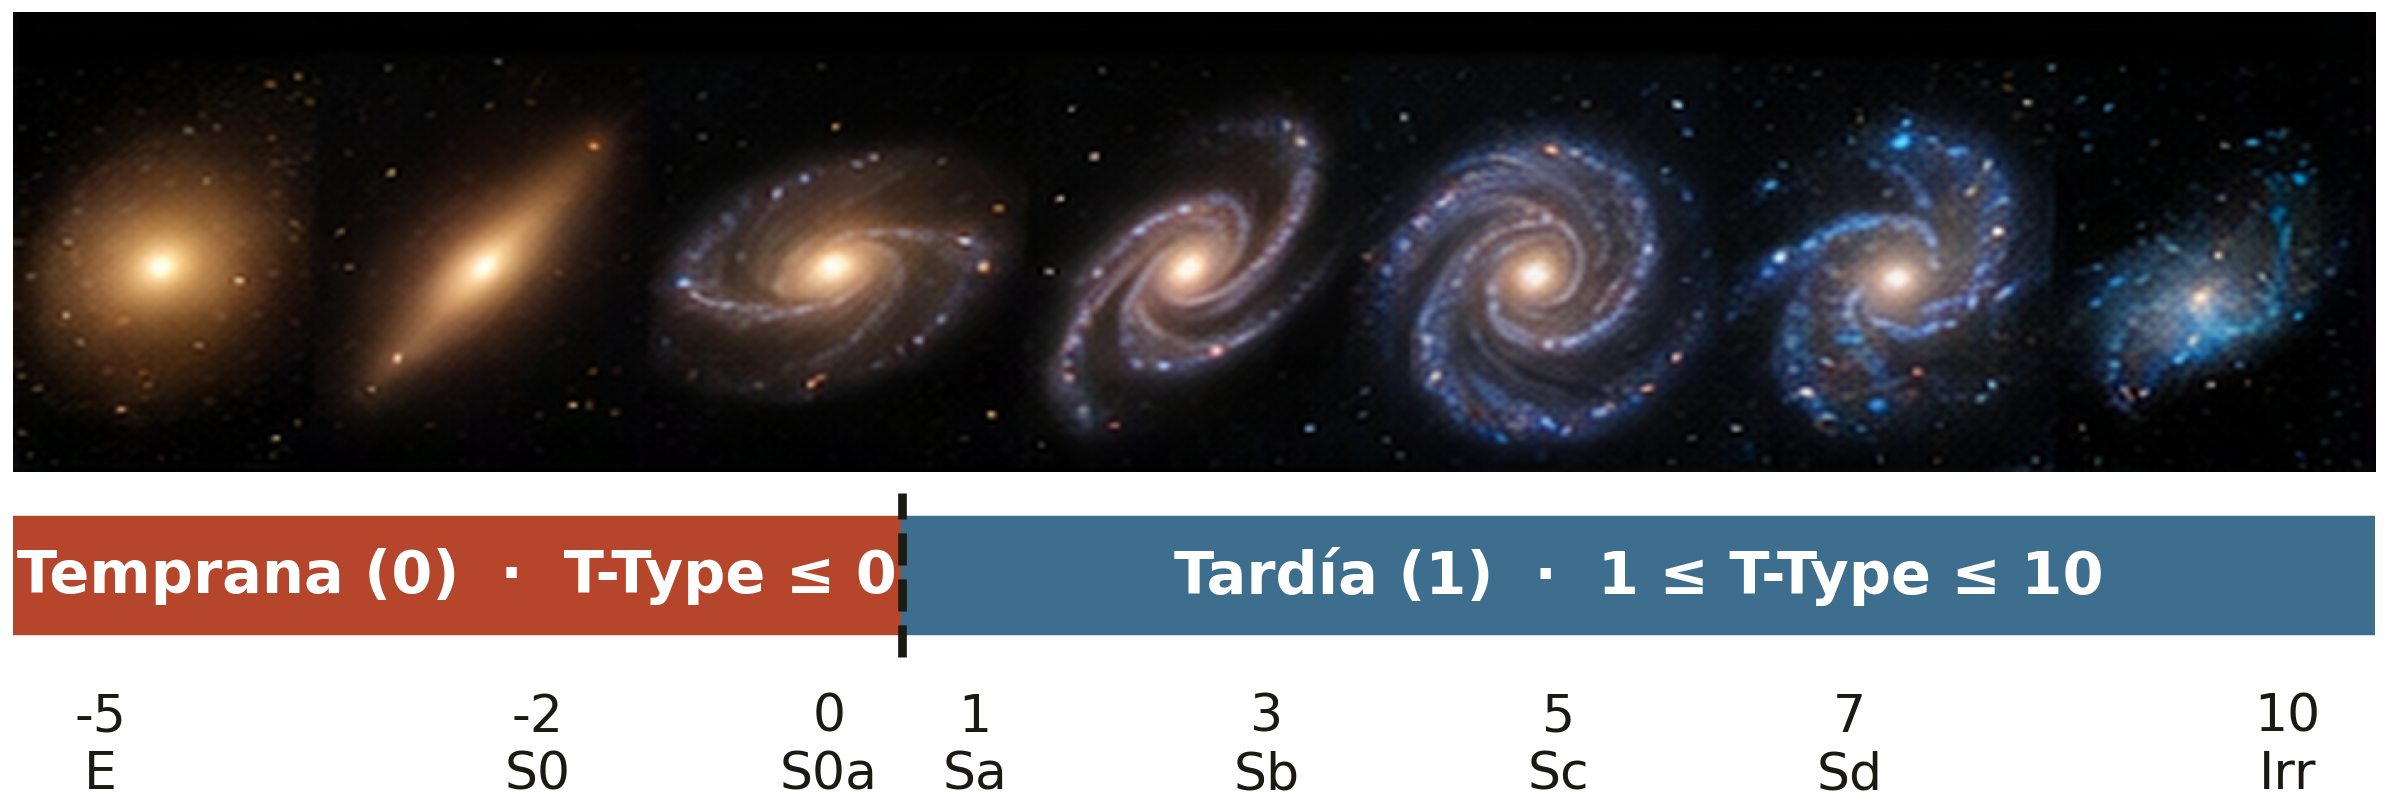
\includegraphics[width=\linewidth]{figs/f1_hubble_ttype.png}\\[2pt]
  \pie{Figura 1. Secuencia de Hubble y etiqueta binaria derivada del T-Type.}
\end{center}
\vfill
\seccion{Datos y preparación}
\begin{center}
  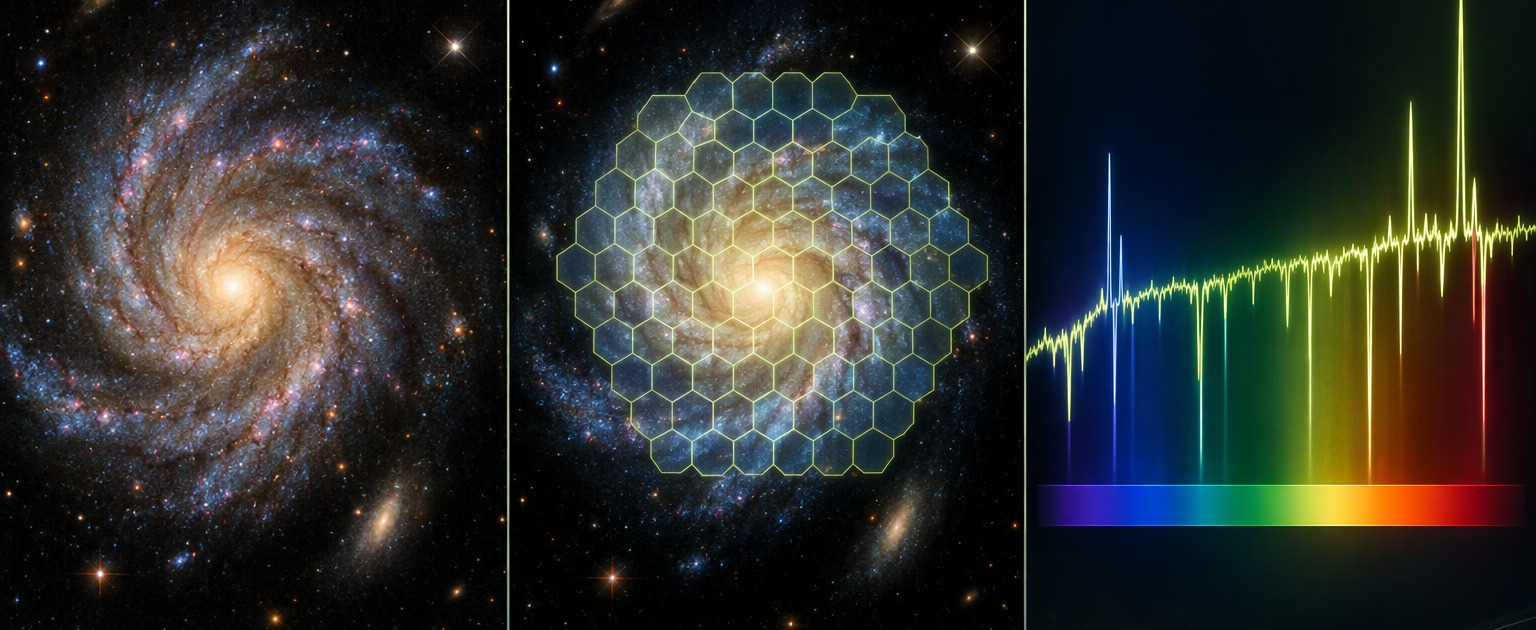
\includegraphics[width=\linewidth,height=4.8cm,keepaspectratio]{figs/modalidades.jpg}\\[2pt]
  \pie{Figura 2. Imagen \textit{grz}, IFU MaNGA, espectro.}
\end{center}
\begin{itemize}
  \item Cut-outs $\propto$ de PETRO\_TH90. Espectro con 4,096 muestras. 90 fracciones del continuum modelado con STARLIGHT.
  \item Máscara descartada, costaba 0.10--0.15 de AUC.
\end{itemize}
\begin{center}
  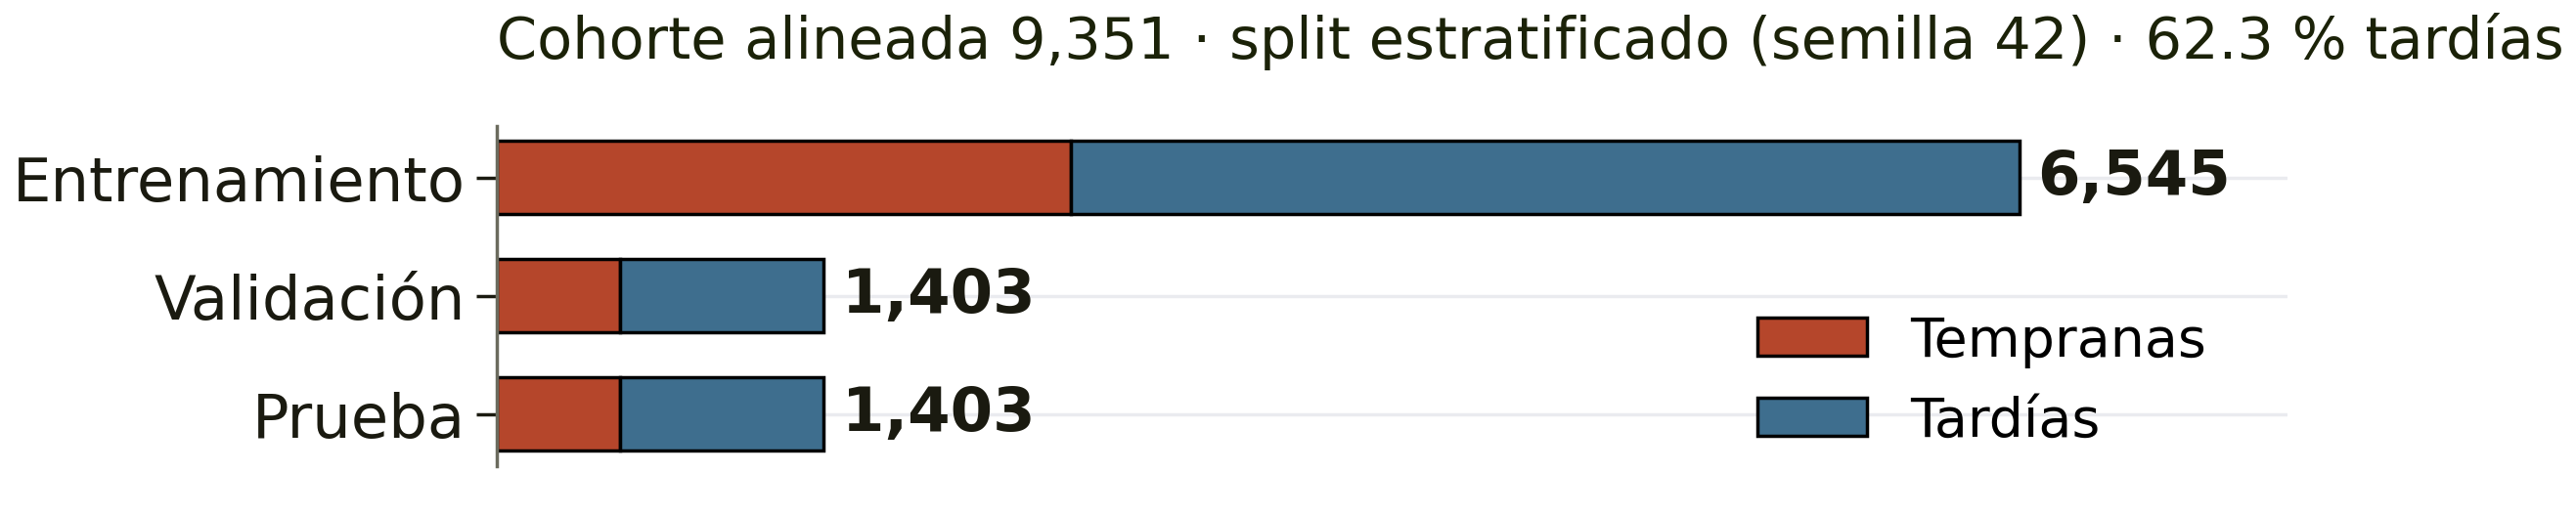
\includegraphics[width=\linewidth]{figs/f2_cohorte.png}
\end{center}
\vfill
\seccion{Metodología: CRISP-ML(Q)}
\begin{center}
  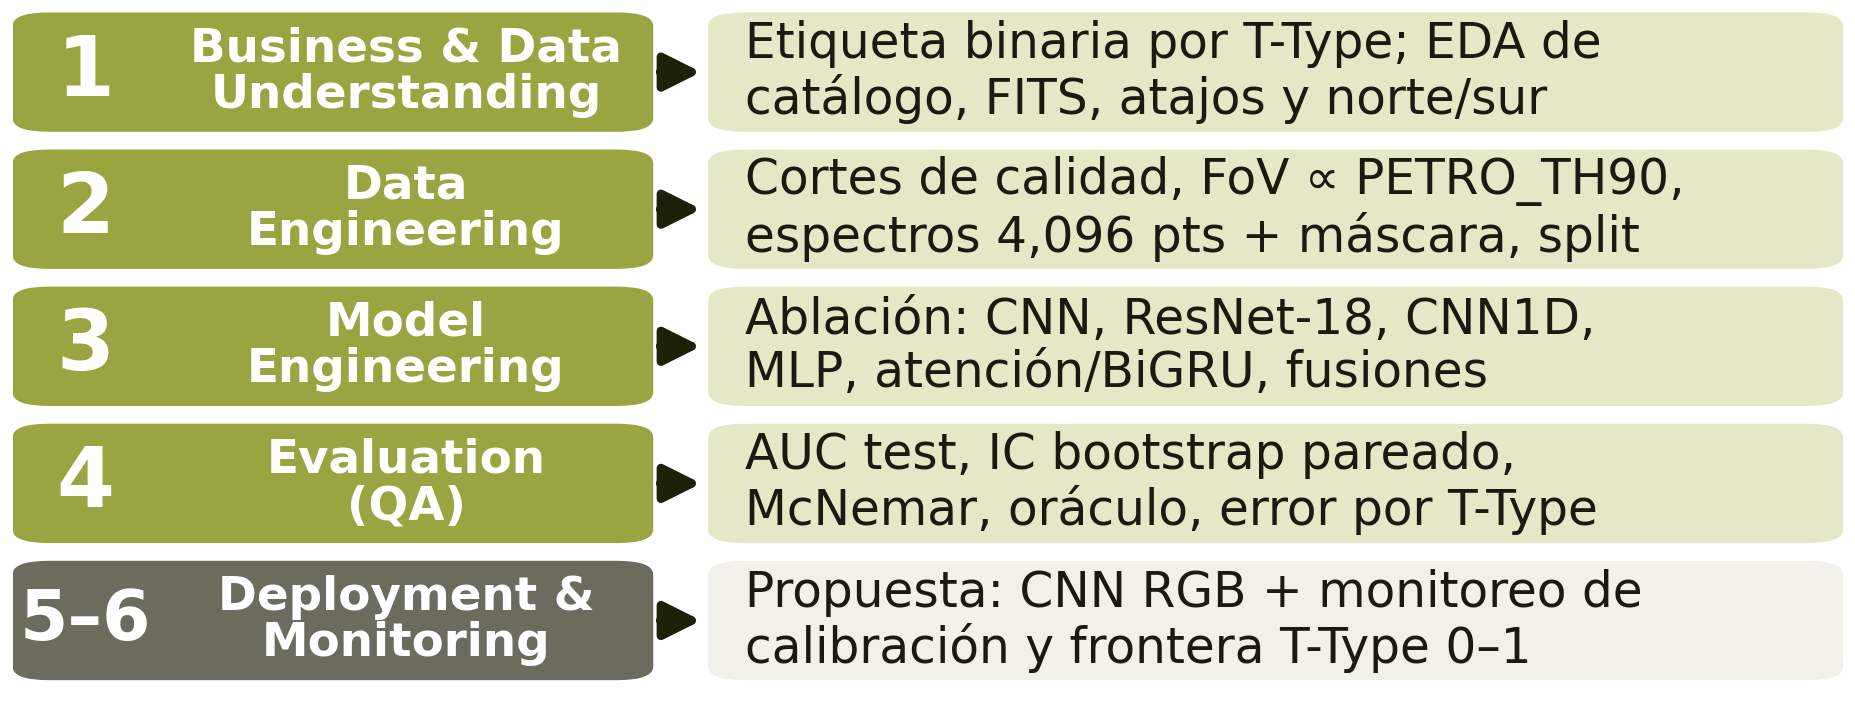
\includegraphics[width=\linewidth]{figs/f3_crisp.png}\\[2pt]
  \pie{Figura 3. Mismo split y protocolo; test evaluado una sola vez.}
\end{center}
\end{minipage}\hfill
\begin{minipage}[t][\colh][s]{0.37\linewidth}\cuerpo\vspace{0pt}
% ===== COLUMNA CENTRAL =====
\noindent\kpi{0.9667}{ROC-AUC\\Modelo Seleccionado}{olivesoft}\hfill
\kpi{89.5\%}{Exactitud\\Balanceada 89.8\%}{olivesoft}\hfill
\kpi{+6.6\,pp}{Sobre el umbral anterior}{olivesoft}\hfill
\kpi{9,351}{Galaxias}{olivesoft}
%\noindent\kpi{0.9667}{ROC-AUC}[MODELO SELECCIONADO]{olivesoft}\hfill 
%\kpi{89.5\%}{Exactitud}[BALANCEADO 89.8\%]{olivesoft}\hfill 
%\kpi{+6.6\,pp}{Sobre el umbral}{olivesoft}\hfill 
%\kpi{9,351}{GALAXIAS}{olivesoft}
\vfill
\seccion{Resultados: La imagen domina el rendimiento}
\begin{center}
  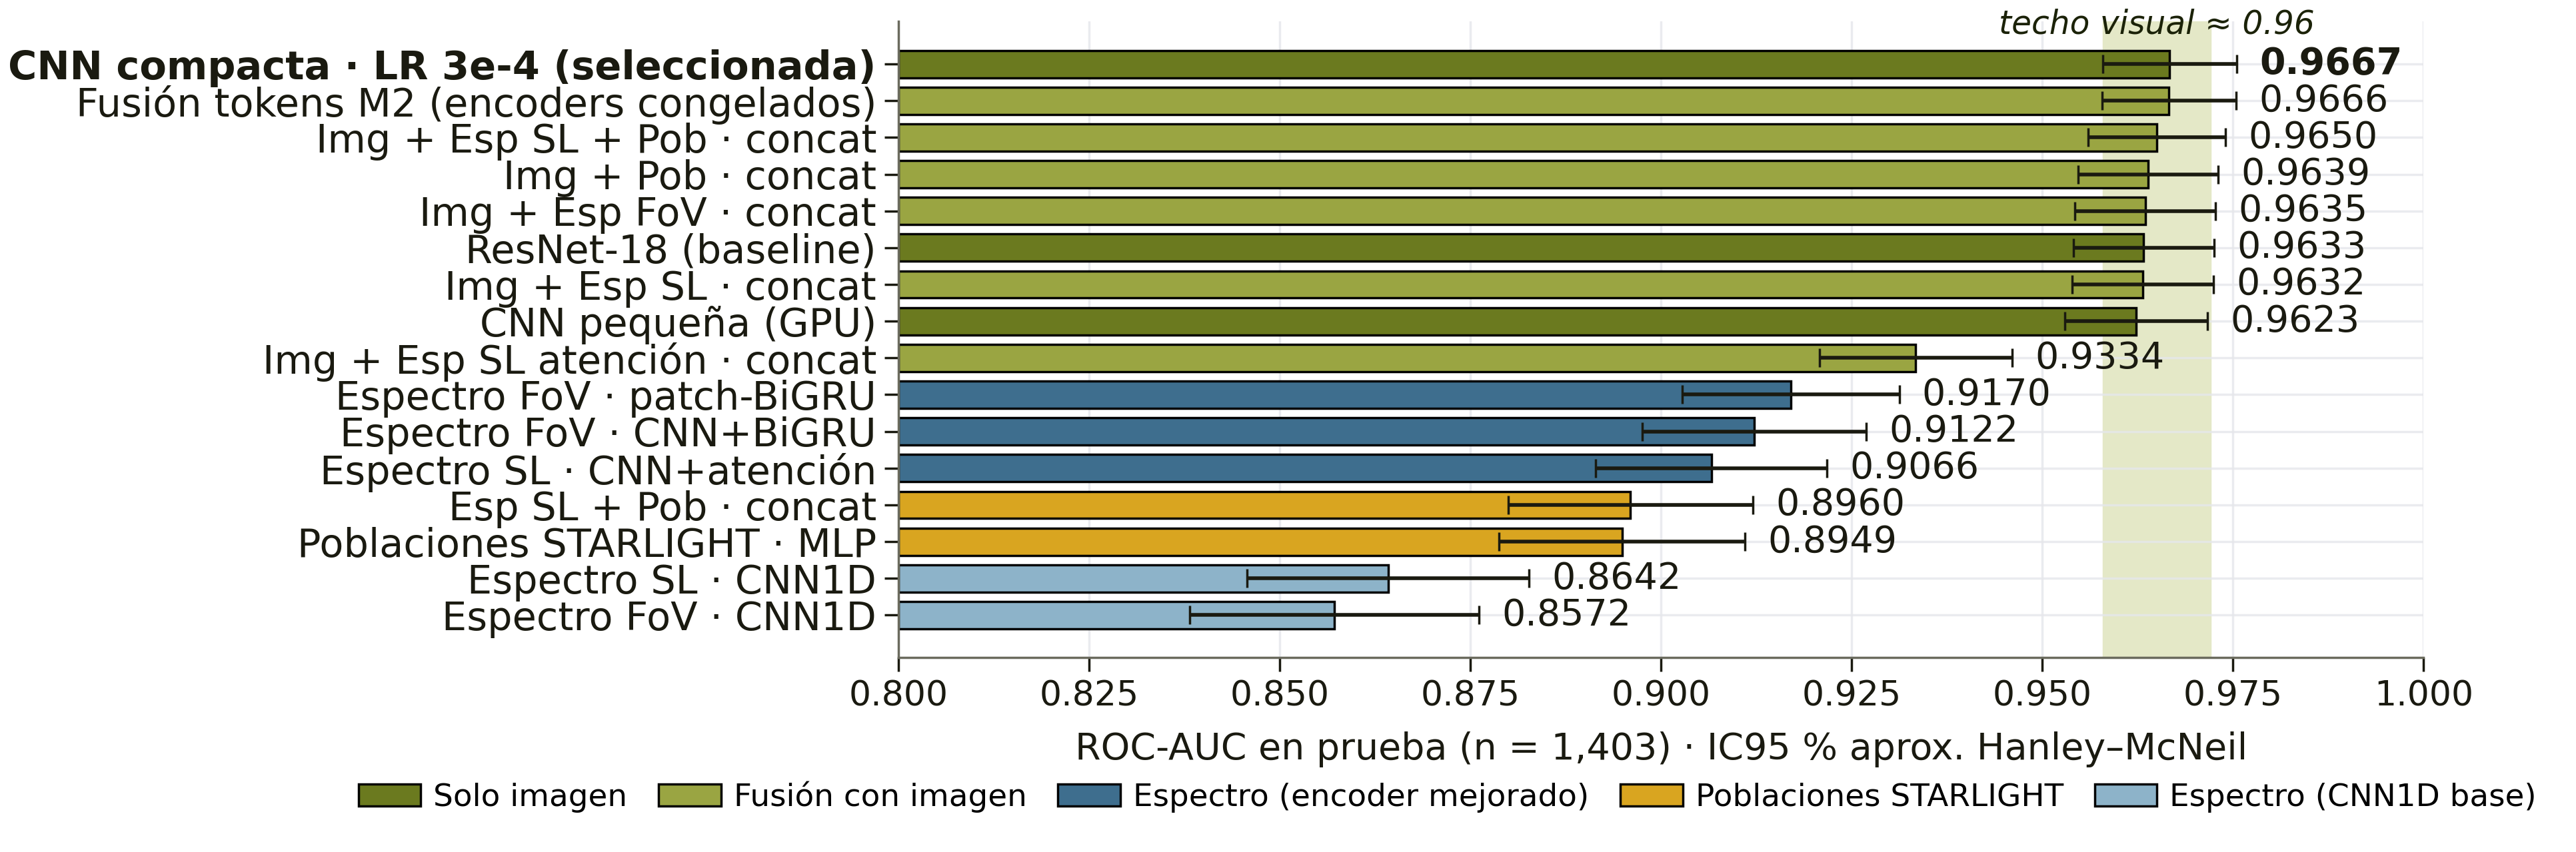
\includegraphics[width=\linewidth]{figs/f4_auc.png}\\[2pt]
  \pie{Figura 4. AUC con una semilla. Solo imagen, 0.962--0.967: diferencias dentro del ruido ($\pm$0.005).}
\end{center}
\vfill
\seccion{El espectro tenía señal solo faltaba extraerla}
\begin{center}
  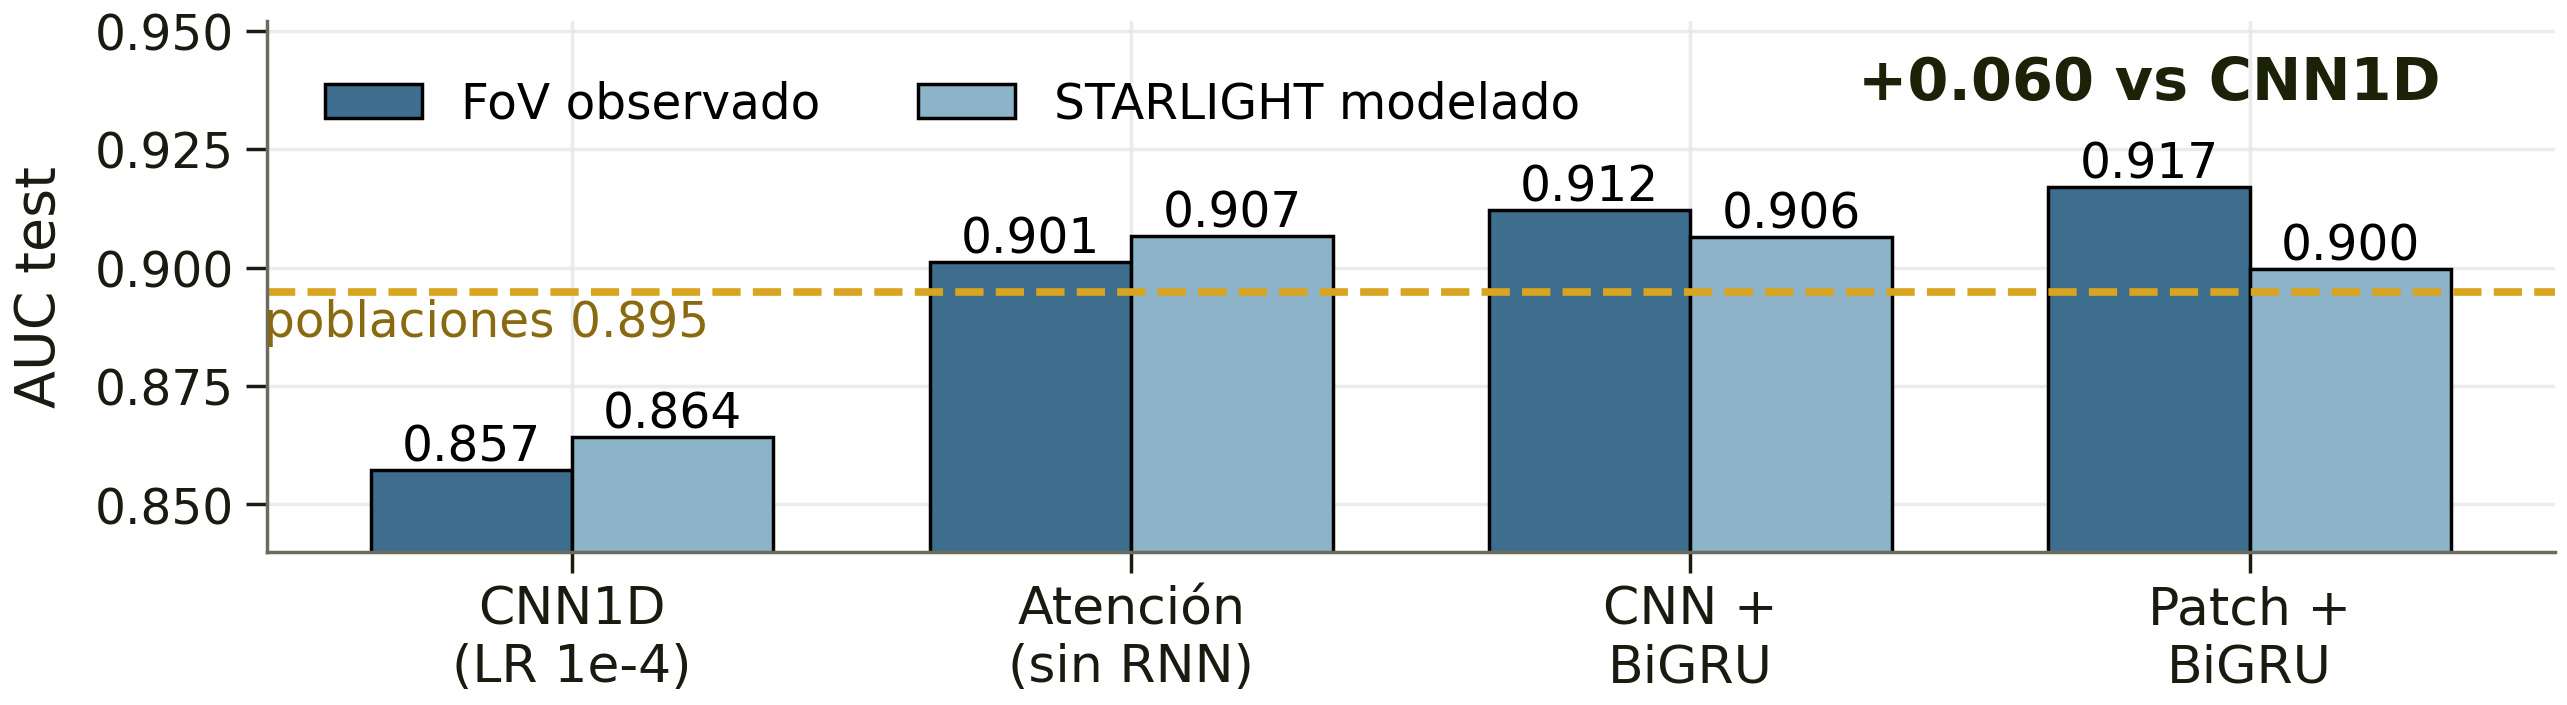
\includegraphics[width=\linewidth]{figs/f5_espectro.png}\\[2pt]
  \pie{Figura 5. LR 3e-4 + \textit{clipping} + más capacidad; la atención sin RNN mejora la predicción.}
\end{center}
\vfill
\seccion{Complementar $\neq$ Fusión}
\begin{center}
  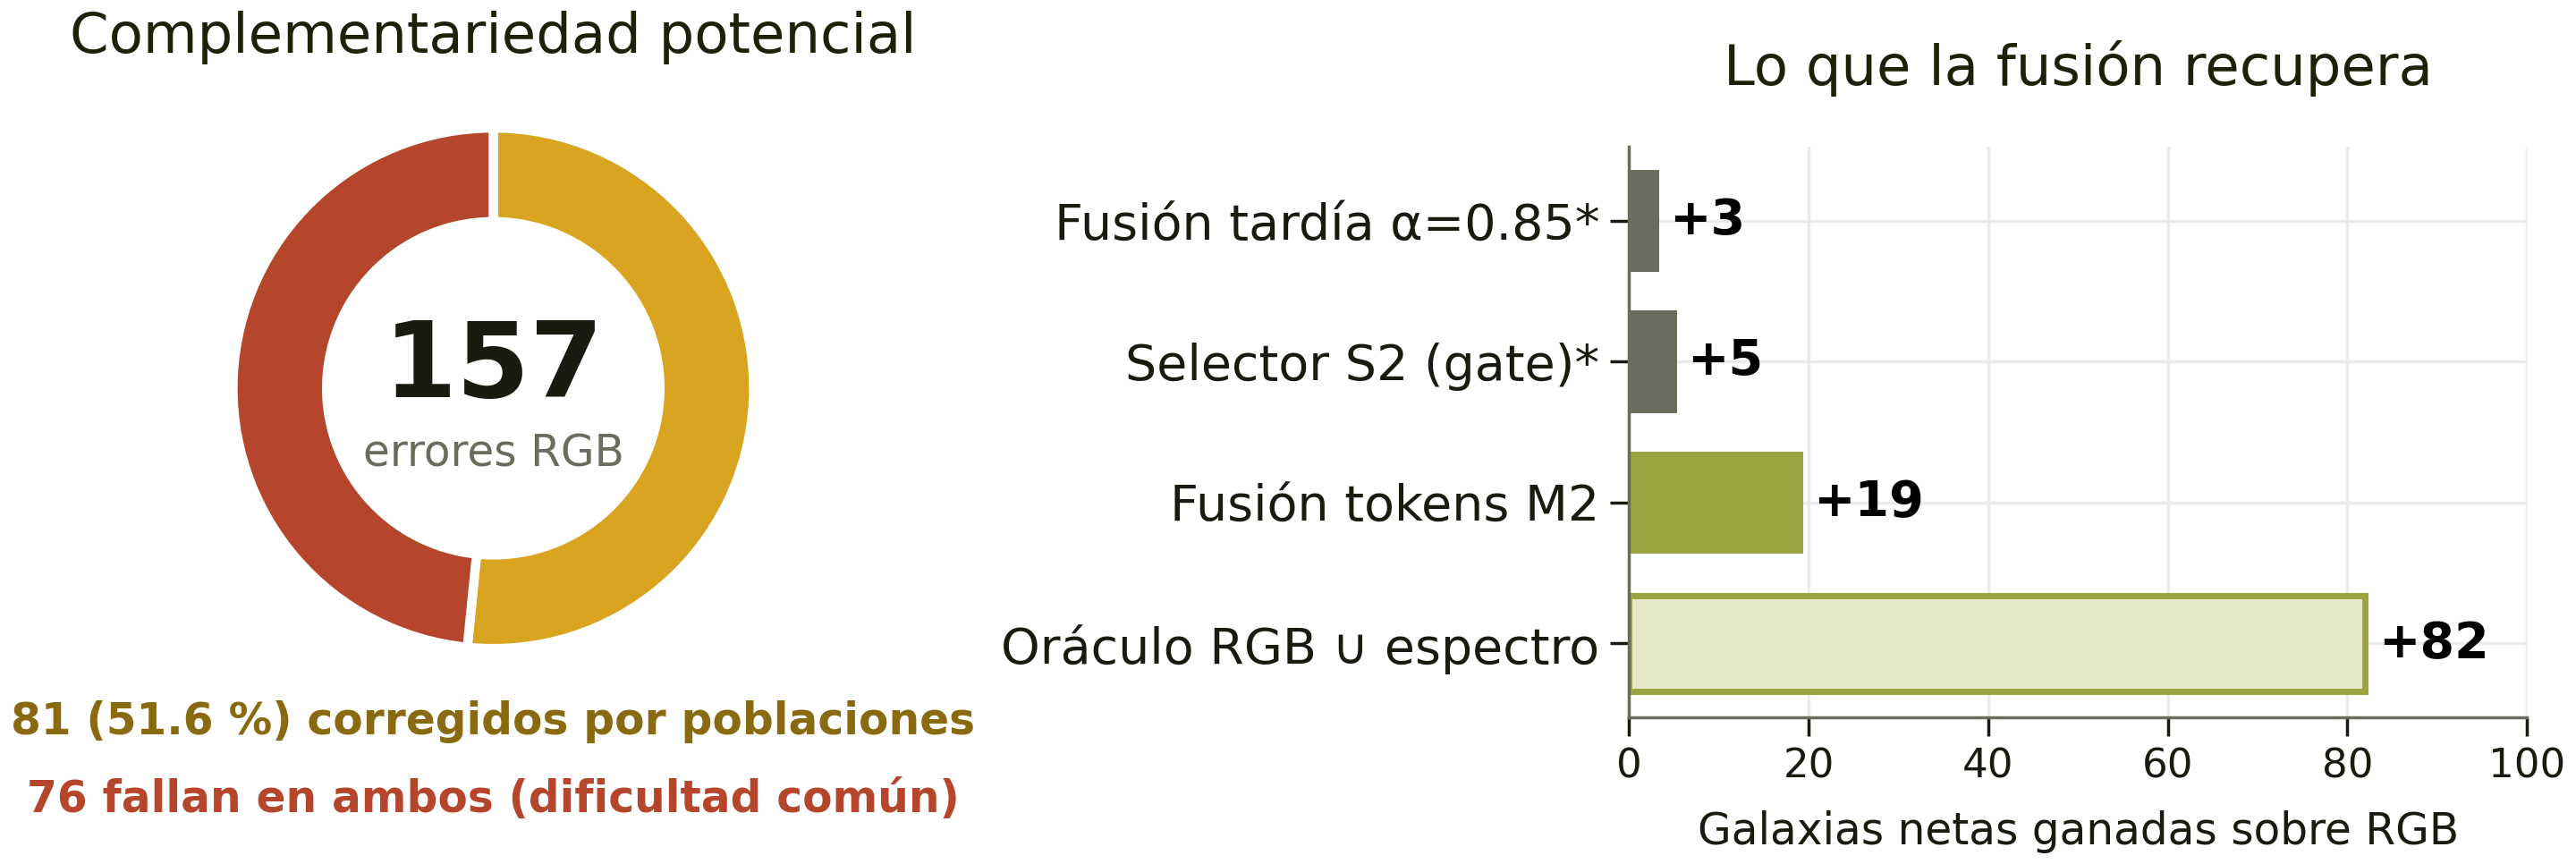
\includegraphics[width=\linewidth]{figs/f6_complementariedad.png}\\[2pt]
  \pie{Figura 6. Ninguna fusión aprovecha más del 23\% del margen del oráculo.}
\end{center}
\end{minipage}\hfill
\begin{minipage}[t][\colh][s]{0.30\linewidth}\cuerpo\vspace{0pt}
% ===== COLUMNA DERECHA =====
\seccion{¿Dónde falla el modelo?}
\begin{center}
  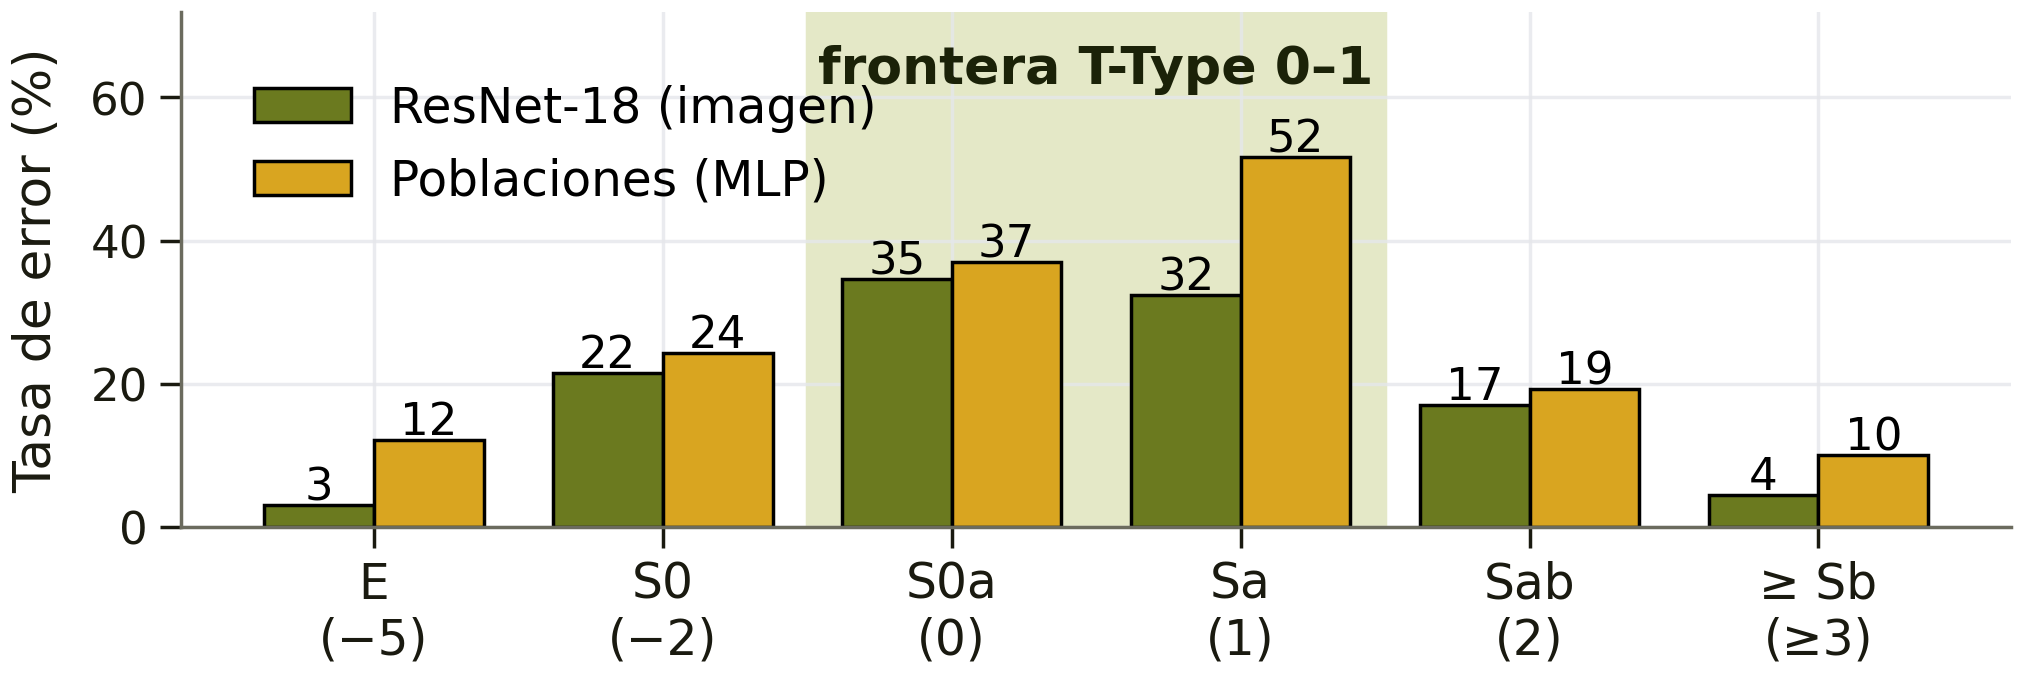
\includegraphics[width=\linewidth]{figs/f7_ttype.png}\\[2pt]
  \pie{Figura 7. Tasa de error por T-Type.}
\end{center}
\clave{T-Type 0--1: Son el \textbf{16\%} de las galaxias, también son el \textbf{48\%} de los errores. Transición física entre S0a y Sa.}
\vfill
\seccion{Conclusiones clave}
\begin{center}
{\sffamily\fontsize{18}{22}\selectfont\color{muted}Tabla 1. Modelo seleccionado frente a referencias (prueba).}
\vspace{0.3em}

\fontsize{22}{28}\selectfont
\renewcommand{\arraystretch}{1.3}
\arrayrulecolor{olivedark}
\begin{tabular}{lccc}
  \toprule
  \textbf{Modelo} & \textbf{AUC} & \textbf{Exactitud} & \textbf{Bal.} \\
  \midrule
  Umbral heredado & -- & 0.829 & -- \\
  ResNet-18 (baseline) & 0.9633 & 0.888 & 0.883 \\
  Fusión tokens M2 & 0.9666 & 0.902 & -- \\
  \rowcolor{olivesoft}\textbf{CNN compacta} & \textbf{0.9667} & \textbf{0.895} & \textbf{0.898} \\
  \bottomrule
\end{tabular}
\end{center}
\begin{itemize}
  \item Desplegar \textbf{CNN RGB} (1.2\,M parámetros).
  \item Fusionar no basta hay que aprender \emph{cuándo} confiar en cada experto.
  \item Límite: una semilla $\Delta$AUC $<$\,0.005 no ordena modelos.
\end{itemize}
\vfill
\seccion{Trabajo futuro}
\begin{center}
  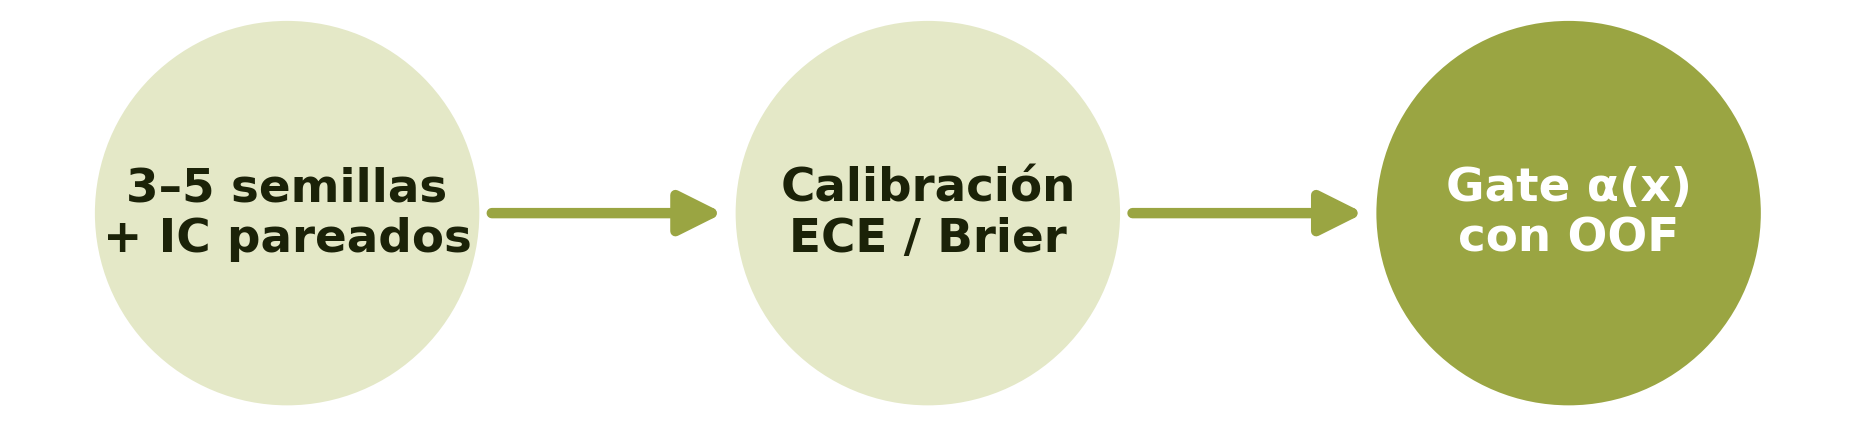
\includegraphics[width=\linewidth]{figs/f8_futuro.png}
\end{center}
\vspace{-0.4em}
\begin{center}
$p_{\mathrm{final}} = \alpha(x)\,p_{\mathrm{RGB}} + [1-\alpha(x)]\,p_{\mathrm{experto}}$
\end{center}
\vfill
\seccion{Referencias}
{\fontsize{18}{23}\selectfont
\begin{itemize}[leftmargin=1.2em,itemsep=0.3em]
  \item Vázquez-Mata, J. A., et al. (2025). \emph{Visual morphological classification of the full MaNGA DR17 sample.} MNRAS, 544(1), 1056--1084.
  \item Studer, S., et al. (2021). \emph{Towards CRISP-ML(Q): A machine learning process model with quality assurance methodology.} MAKE, 3(2), 392--413.
  \item He, K., Zhang, X., Ren, S., y Sun, J. (2016). \emph{Deep residual learning for image recognition.} CVPR, 770--778.
\end{itemize}}
\end{minipage}
\vfill
% ---------------------- DECLARACIÓN DE IA ------------------
{\color{olive}\rule{\linewidth}{2.5pt}}
\vspace{0.3cm}
\noindent
{\fontsize{18}{23}\selectfont\color{ink}
{\serif\color{olivedark}\fontsize{22}{28}\selectfont Declaración de uso de inteligencia artificial.}
Se uso Microsoft Copilot (basado en Claude) para la síntesis y revisión de redacción, el formato del póster en \LaTeX{}, la generación de las gráficas a partir de métricas, y la generación de imágenes (Figuras 1 y 2).\par}
\end{document}
